Until now we have described the bootware in a generic context because it should work with various different SWfMSs.
But for the implementation we will have to work with a specific system, which in our case is the SimTech SWfMS.
\autoref{image:generic} shows the bootware being used together with the SimTech SWfMS.
It also shows the components as one of three types: specific, generic, and adapted.
The specific components, shown in black, are those components that belong to a specific SWfMS.
In our case these are the SimTech Modeler at the bottom left and the SimTech ODE (and other components that were omitted in this figure) in the center.
On the other hand we have the generic components, shown in white.
These are components that are build to be generic and can be used in all kinds of environments.
In our case these are the local and remote bootwares and their plugins, as well as the provisioning manager and the ESB (here Apache Service Mix) and various repositories and registries.
The specific and the generic components have to work together, but there should be no need to make huge modifications to either one to do so.
Therefore, we need adapter components in some places, which are shown in gray in \autoref{image:generic}.
They are responsible for gluing together specific and generic components where necessary and should be the only components that have to be modified or created from scratch to fit to a specific environment.
In our case this is the bootware plugin, an implementation of the bootware adapter described in \autoref{design:modeler_integration}, loaded in the SimTech Modeler on the bottom left.
There also is an adapter component between the SimTech ODE and Apache Service Mix, which is not shown here.

\begin{figure}[!htbp]
	\centering
	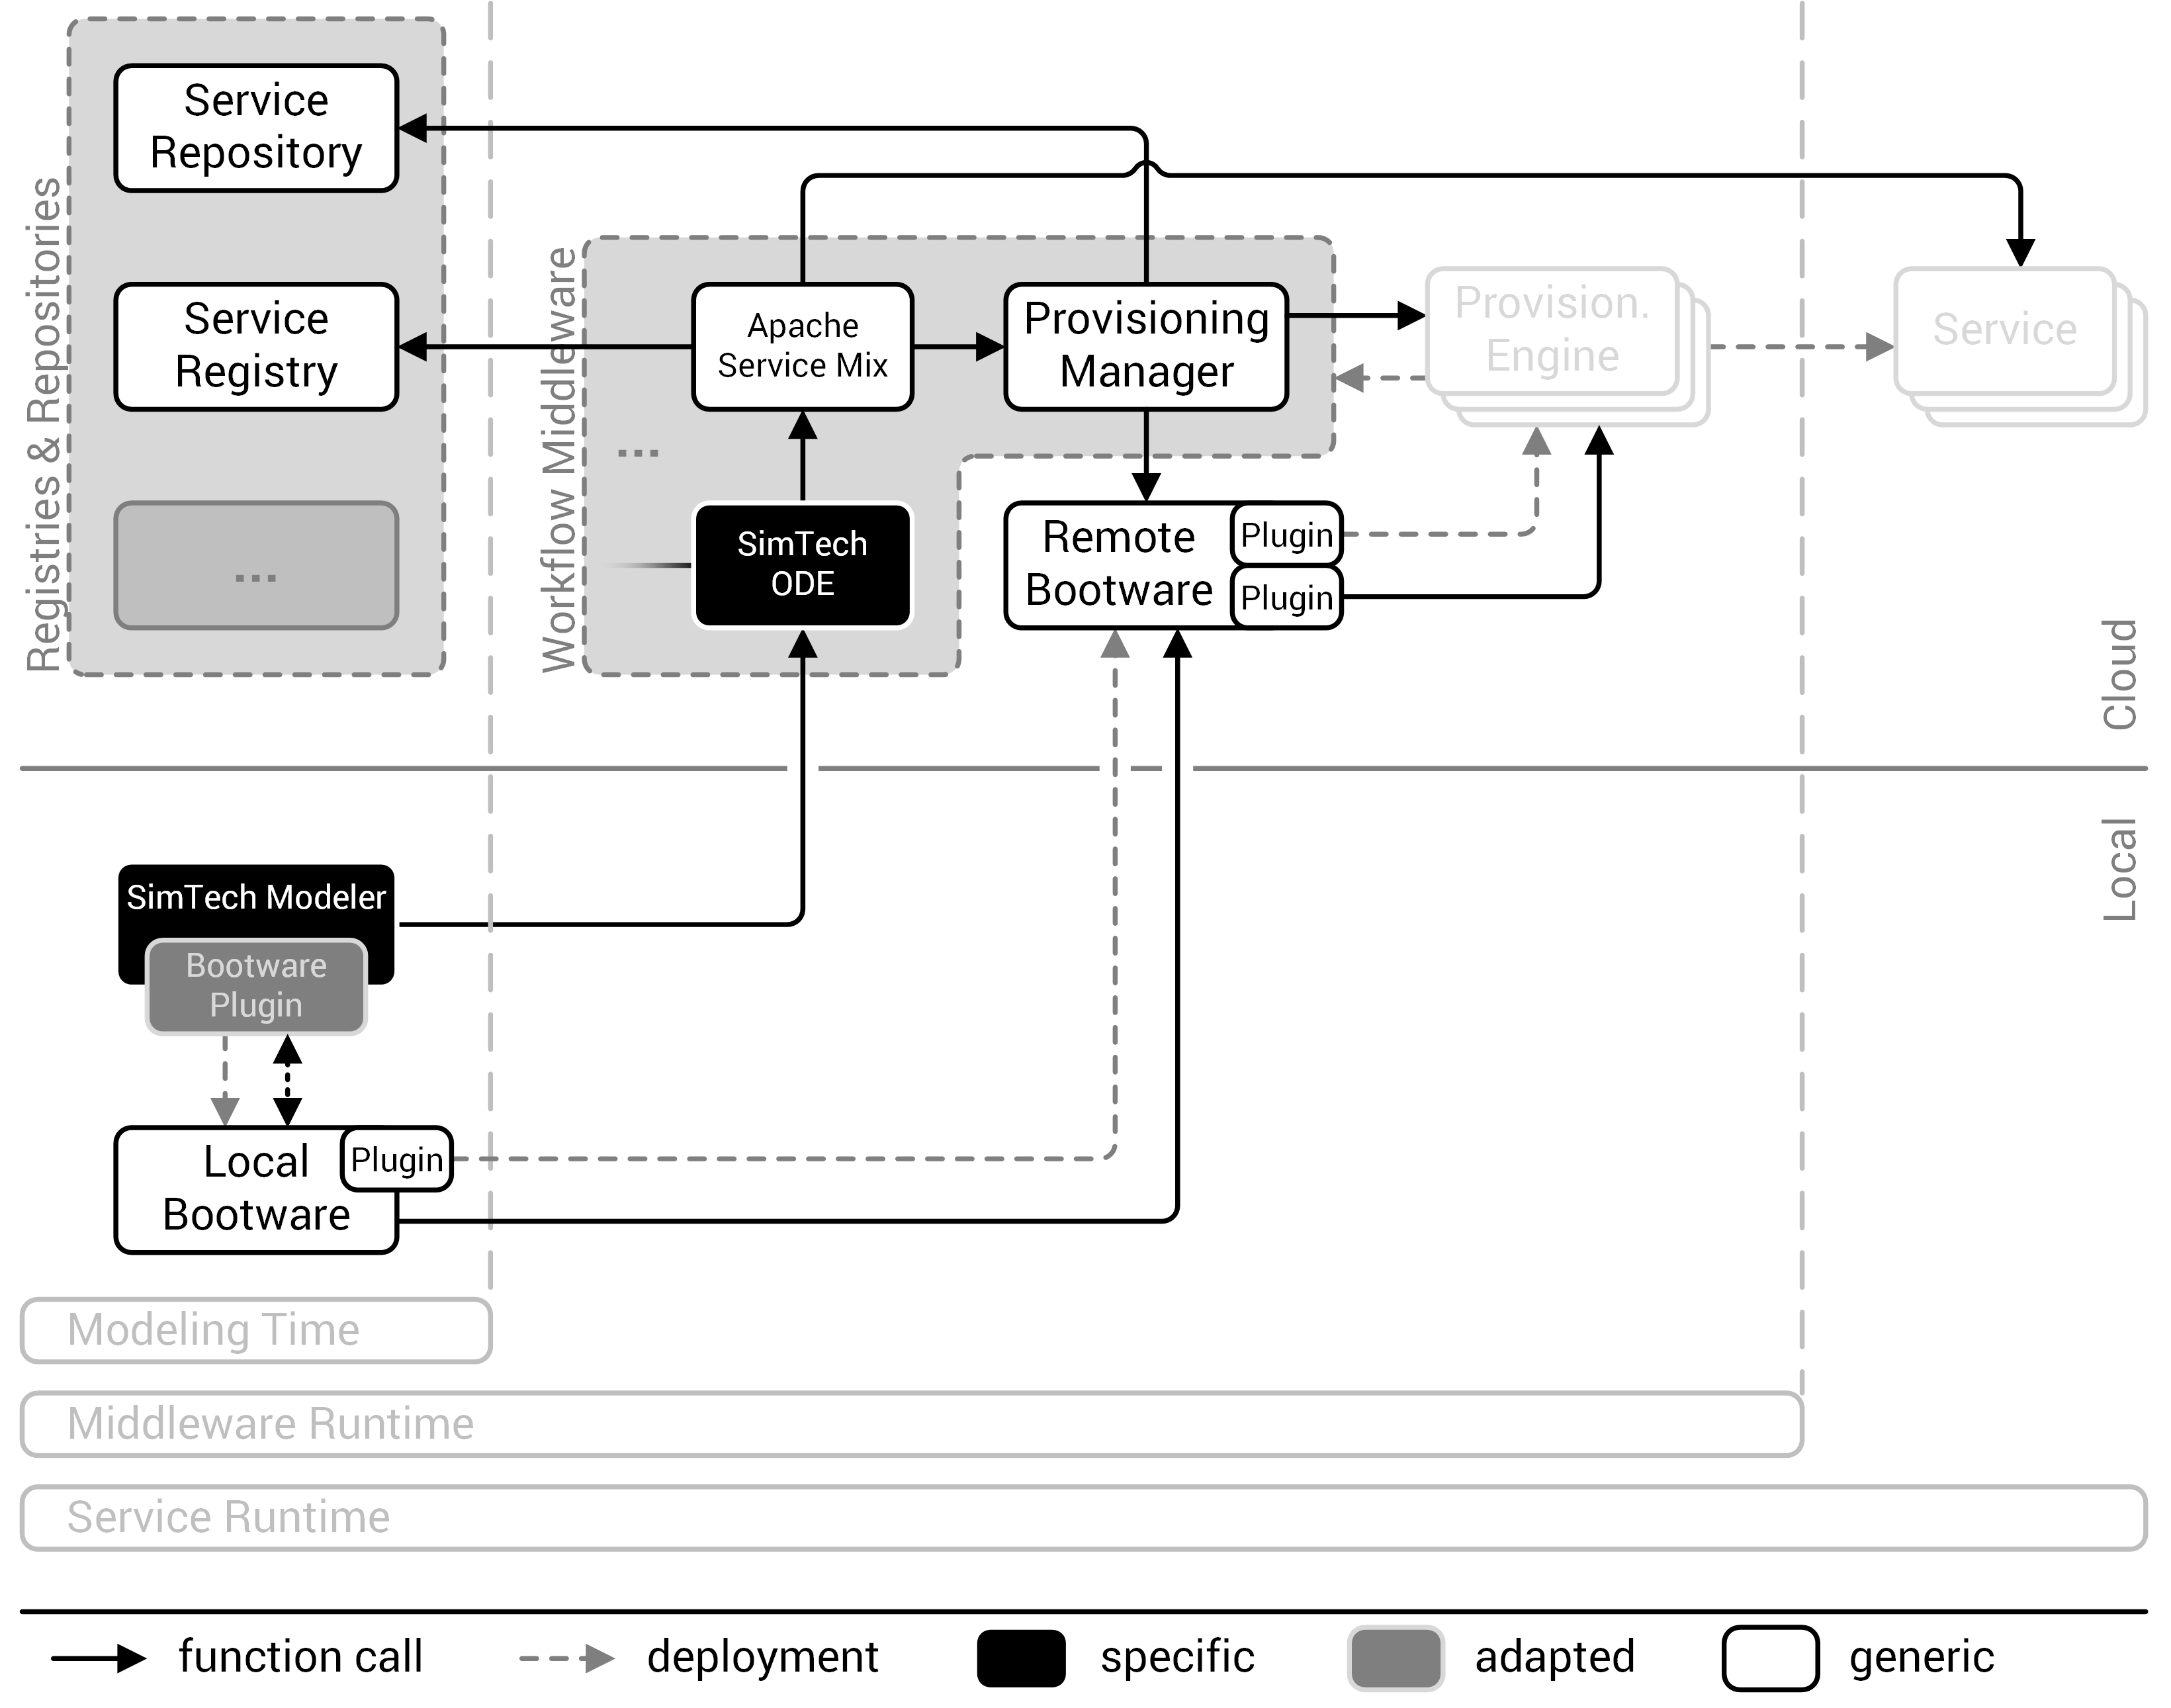
\includegraphics[resolution=600]{implementation/assets/generic}
	\caption{Specific and generic components and adapters.}
	\label{image:generic}
\end{figure}

For the implementation of this diploma thesis we will have to create the generic local and remote bootware components and their plugins, as well as the bootware plugin, which will be specific to the SimTech Modeler.
In the rest of the chapter we present details on the implementation of the bootware components.
First, we describe the implementation of the bootware plugin.
Next, we select specific frameworks and libraries that allow us to implement the architecture we developed in \autoref{design}.
Then, we present detailed descriptions of the implementation of some parts of the local and remote bootware and some plugins.
